\subsection{Kubernetes}
\subsubsection{Kubernetes Architecture}
\begin{figure}[ht]
    \begin{center}
        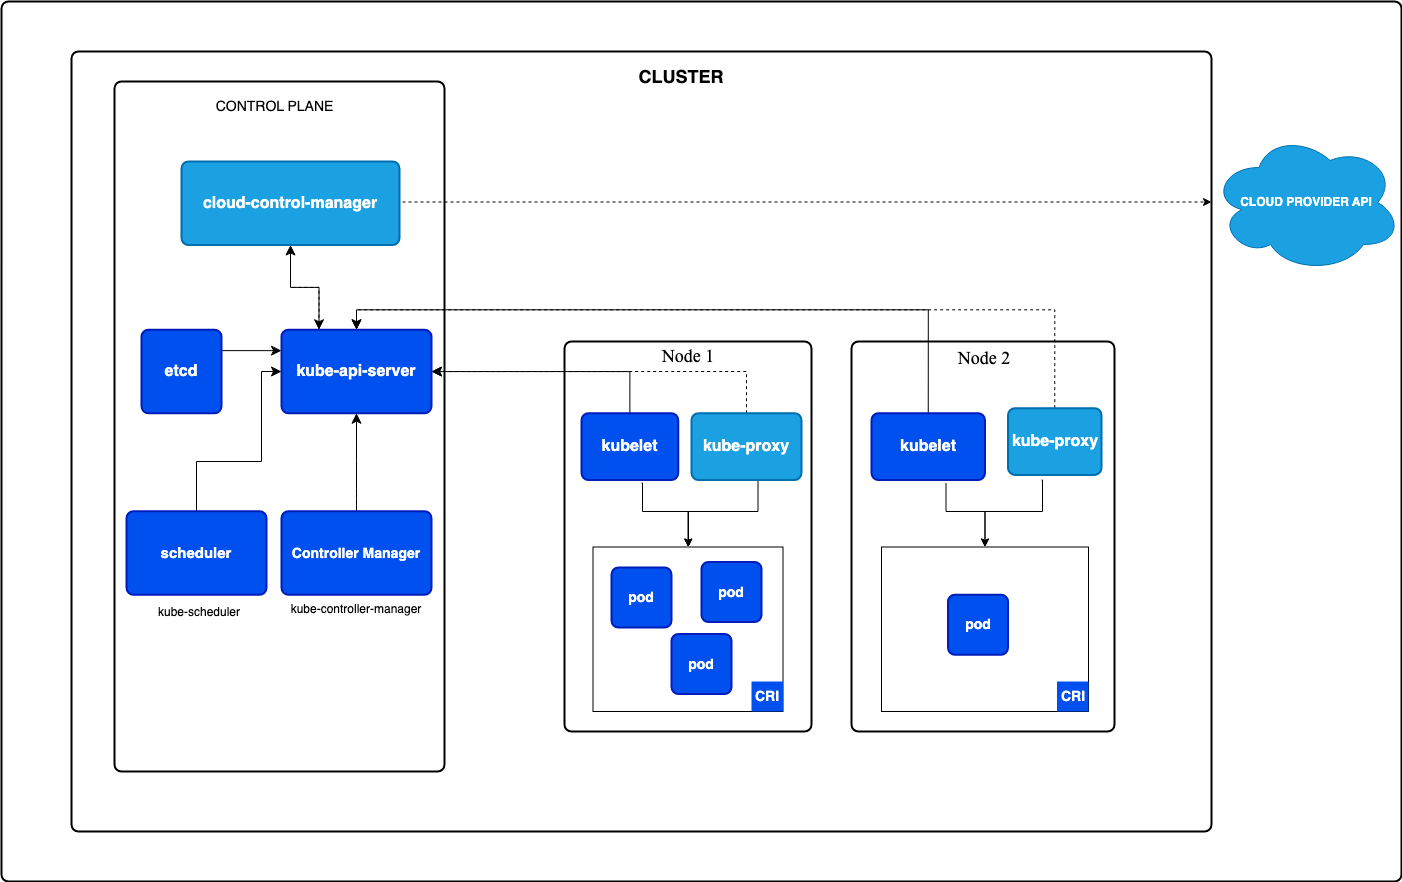
\includegraphics[scale=0.2]{images/kube_arc.png}
    \end{center}
    \caption[แผนผังแสดงโครงสร้างของ Kubernetes]{แผนผังแสดงโครงสร้างของ Kubernetes}
\end{figure}

แต่ละ Cluster มีสามส่วนประกอบหลักที่ต้องรู้ก่อนทำงานกับ K8s:
\begin{itemize}
    \item \textbf{Master Node (Control plane)}: ควบคุมและจัดการการดำเนินงานทั้งหมดใน K8s มีองค์ประกอบหลัก 3 ตัวดังนี้:
          \begin{itemize}
              \item \textbf{kube api server:} ทำหน้าที่เป็นตัวกลางในการสื่อสารภายใน Cluster ผ่าน RESTful API
              \item \textbf{kube scheduler:} ทำหน้าที่เป็นผู้จัดการ Pod เมื่อมี Pod ใหม่เข้ามา จะค้นหา Worker Node ที่เหมาะสมสำหรับ Pod ที่กำลังจะเข้ามาใหม่โดยต้องใช้ข้อมูลจากหลายแหล่งเพื่อทำการตัดสินใจ
              \item \textbf{kube controller manager:}
                    \begin{itemize}
                        \item \textbf{Node Controller:} ควบคุม Node
                        \item \textbf{Replication Controller:} จัดการการจำลอง Pod
                        \item \textbf{Endpoints Controller:} ควบคุม Endpoint
                        \item \textbf{Service Account \& Token controllers:} จัดการ Service Account และ API Access Token
                    \end{itemize}
              \item \textbf{cloud controller manager:} ตัวควบคุมนี้จะมีเฉพาะใน Cloud Provider ที่รองรับ K8s ทำหน้าที่คล้ายกับ kube controller manager แต่ทำงานร่วมกับ Cloud Provider แต่ละเจ้าโดยตรง
          \end{itemize}
          \clearpage
    \item \textbf{Worker Node}: คอนเทนเนอร์รันไทม์รวมถึงสองบริการ:
          \begin{itemize}
              \item \textbf{kubelet:} รับคำสั่งจาก kube api server และจัดการ Container runtime เช่น ตรวจสอบว่า Pods ยังคงทำงานบน Worker Node หรือไม่ หากมีปัญหาจะรายงานไปยัง kube api server เพื่อจัดการ Pods ใหม่อีกครั้ง
              \item \textbf{kube proxy:} บริการนี้ช่วยให้ Pods สามารถเชื่อมต่อจากภายนอกคลัสเตอร์ได้ ทำหน้าที่เหมือนพร็อกซีเซิร์ฟเวอร์ในการรับคำขอจากภายนอกและส่งต่อไปยัง Pods ที่เหมาะสมภายใน Node
          \end{itemize}

    \item \textbf{etcd}: ใช้สำหรับจัดเก็บสถานะ Cluster (Persistent Cluster State) ซึ่งเป็นส่วนหนึ่งของ Control Plane ที่เชื่อมต่อโดยตรงกับ kube api server
\end{itemize}
